\documentclass{beamer}
\usetheme[compress]{Padova}
\usepackage{packages}
\usepackage{statmacros}
\title{\textsc{Clustering distribuito tramite MapReduce}}
\author{\centering Daniele Zago \and Giovanni Toto}
\date{\mbox{}\\[2cm]\today}

% Separatore di argomenti
\newcommand{\separator}[1]{
\begin{frame}[sep]
\centering
\vspace*{\fill}
{\color{white}\huge #1}
\vspace*{\fill}
\end{frame}
}

\usepackage{verbatim} %commenti

\begin{document}
\begin{frame}
\titlepage
\end{frame}


\begin{frame}{MapReduce}
    \emph{MapReduce} è un framework per la creazione di applicazioni in grado di elaborare grandi quantità di dati in parallelo.
    \\[.5cm]
    Fornisce un'astrazione che nasconde al programmatore la complessità derivante dalla parallelizzazione.
    \pause\\[.5cm]
    E' necessario solo definire una serie di processi intermedi, che ricevono e ritornano dati nella forma $\langle \textit{chiave, valore} \rangle$:
    \\[.5cm]
    \begin{itemize}
        \item[-] funzione \emph{map}:\\ riceve in input una singola osservazione
        \item[-] funzione \emph{reduce}:\\ per ogni chiave, elabora i valori ad essa associati e ritorna il risultato finale dell'intero processo
    \end{itemize}
\end{frame}


\begin{frame}{Cluster Analysis}
    L'analisi dei gruppi (\textit{cluster analysis}) è un insieme di metodi che suddividono l'insieme di dati $\mathcal{X}$ in sottoinsiemi i cui membri risultano \textit{simili} tra loro.
    \\[.5cm]
    I metodi proposti interpretano i dati $x$ come vettori di uno spazio vettoriale $\mathcal{X} \subseteq \R^{p}$, sul quale è definita una funzione distanza $d(\cdot, \cdot)$.\\[.5cm]
    \pause
    \textbf{Obiettivo}: creare delle partizioni, o \emph{cluster}, che minimizzino la similarità tra gli elementi appartenenti allo stesso gruppo.
    \\[.5cm]
    I cluster sono rappresentati da centroidi, che riassumono l'informazione contenuta nel dataset.
\end{frame}


\begin{frame}{Algoritmo \km}
    La procedura di raggruppamento porta alla minimizzazione di una funzione obiettivo $\loss(\cdot )$, la cui specificazione dipende dalla distanza $d(\cdot , \cdot )$ e dal numero di cluster $k$:
    \\[.5cm]
    \[
    \loss(c_1, \ldots, c_k) = \sum_{j=1}^{k} \sum_{x_i \in R_k} d(x_i, c_j)^2 
    \]
    Scegliendo la norma euclidea, si ha una soluzione esplicita:
    \[
        c_j = \frac{1}{|R_j|}\sum_{x \in R_j} x, \quad j=1, \ldots, k
    \]
\end{frame}


\begin{frame}{Algoritmo \km}
    L'algoritmo di stima, ad ogni iterazione, alterna due passaggi:\\[.5cm]
    \begin{itemize}
        \item[1.] ogni punto è assegnato al cluster più vicino
        \item[2.] i centroidi sono aggiornati tramite
        \[
        c_j = \frac{1}{|R_j|}\sum_{x \in R_j} x, \quad j=1, \ldots, k
        \]
    \end{itemize}
    % \\[.5cm]
    Iterando fino a convergenza, è possibile ottenere un minimo locale della funzione $\loss(c_1, c_2, \ldots, c_k)$.
\end{frame}


\begin{frame}{Algoritmo \km}
    \begin{algorithm}[H]
        \caption{\km\ \textit{map}}
        \begin{algorithmic}[1]
            \setstretch{1.15}
            \Require $c_1, c_2, \ldots, c_k, x_i$
            \Ensure $\big\langle j, x_i \big\rangle $
            \State $j \leftarrow \argmin_{h = 1, \ldots, k} d(x, c_h)$
            \State \Return $\big\langle j, x \big\rangle $
        \end{algorithmic}
    \end{algorithm}
    \begin{algorithm}[H]
        \caption{\km\ \textit{reduce}}
        \begin{algorithmic}[1]
            \Require $\langle j, R_j \rangle $
            \Ensure $\langle j, c_j \rangle $
            \State $c_j \leftarrow \frac{1}{|R_j|}\sum_{x \in R_j} x, \quad j=1, \ldots, k$
            \State \Return $\langle j, c_j \rangle $
        \end{algorithmic}
    \end{algorithm}
\end{frame}


\begin{comment}
\begin{frame}{Algoritmo \km}
\begin{algorithm}[H]
\caption{\km}
\begin{algorithmic}[1]
    \setstretch{1.15}
    \Require $c^{0}_1, c^{0}_2, \ldots, c^{0}_k$
    \While{$\max_j d(c_j^{l+1}, c_j^{l}) > \varepsilon$}
        \For{$j \in 1, \ldots, k$}
        \State $R^{l+1}_j \leftarrow \{x \in \mathcal{X} : \argmin_{h} d(x , c^{l}_h) = j \} $
        \EndFor
        \For{$j \in 1, \ldots, k$}
        \State $c_j^{l+1} \leftarrow \frac{1}{n_j}\sum_{x \in R_j^{l+1}} x $
        \EndFor
    \EndWhile
\end{algorithmic}
\end{algorithm}
\end{frame}
\end{comment}


\begin{frame}{Matrice di Appartenenza}
    Per tenere traccia del grado di appartenenza di ogni osservazione ai vari cluster, si definisce la \emph{matrice di appartenenza} $U = \left( u_{ij} \right)$ soggetta ai vincoli:\\[.5cm]
    \begin{itemize}
        \item[-] $\sum_{j=1}^{k} u_{ij} = 1$, \quad i=1, \ldots, n
        \item[-] $u_{ij} \in \{0,1\}$, \quad i=1, \ldots, n, j=1, \ldots, k
    \end{itemize}
    \pause
    Modificando il secondo vincolo, è possibile generalizzare il \km\ e renderlo un metodo di raggruppamento \emph{fuzzy}:
    \[
    u_{ij} \in \{0,1\} \quad \rightarrow \quad u_{ij} \in [0,1]
    \]
    Così facendo, $u_{ij}$ diventa il peso con cui l'$i$-ma osservazione appartiene al $j$-mo cluster.
\end{frame}


\begin{frame}{Algoritmo \fcm}
    Aggiungendo un ulteriore parametro $m \geqslant 1$, detto \textit{grado di mescolamento}, che determina quanto risulteranno \emph{fuzzy} i \textit{cluster} prodotti, si ottiene l'algoritmo \fcm.
    \\[.5cm]
    Il problema di minimo diventa
    \[
    \loss(c_1, \ldots, c_k) = \sum_{i=1}^{k} \sum_{i=1}^{n} u_{ij}^{m}d(x_i, c_j)^2 ,
    \]
    \\[.5cm]
    da cui si ottiene la soluzione esplicita
    \[
        c_j = \frac{ \sum_{i=1}^{n} u_{ij}^{m} x_i}{\sum_{i=1}^{n} u_{ij}^{m}}, \quad j=1, \ldots, k
    \]
\end{frame}


\begin{frame}{Algoritmo \fcm}
    L'algoritmo di stima, ad ogni iterazione, alterna due passaggi:
    \\[.5cm]
    \begin{itemize}
        \item[1.] la \emph{matrice di appartenenza} è aggiornata tramite
        \[
        u_{ij} = \left(\sum_{h=1}^{k} \Big(\frac{d(x_i, c_j)}{d(x_i, c_h)}\Big)^{\frac{2}{m-1}}\right)^{-1}
        \]
        \item[2.] i centroidi sono aggiornati tramite
        \[
        c_j = \dfrac{\sum_{i=1}^{n} u_{ij}^{m}x_i}{\sum_{i=1}^{n} u_{ij}^{m}}
        \]
    \end{itemize}
    % \\[.5cm]
    Iterando fino a convergenza, è possibile ottenere un minimo locale della funzione $\loss(c_1, c_2, \ldots, c_k)$.
\end{frame}


\begin{frame}
    \begin{algorithm}[H]
        \caption{\fcm\ \textit{map}}
        \begin{algorithmic}[1]
            \setstretch{1.15}
            \Require $c_1, c_2, \ldots, c_k, x_i$
            \Ensure $\big\langle j, (u_{ij}^{m} x_i, u_{ij}^{m}) \big\rangle $ per $j = 1, \ldots, k$
            \For{$j = 1, \ldots, k$}
            \State $d_{ij} \leftarrow d(x_i, c_j)$
            \EndFor

            \For{$j = 1, \ldots, k$}
            \State $u_{ij} \leftarrow \left(\sum_{h=1}^{k} \Big(\frac{d_{ij}}{d_{ih}}\Big)^{\frac{2}{m-1}}\right)^{-1} $
            \State \Return $\big\langle j, (u_{ij}^{m}x_i, u_{ij}^{m}) \big\rangle $
            \EndFor
        \end{algorithmic}
    \end{algorithm}
\end{frame}


\begin{frame}
    \begin{algorithm}[H]
        \caption{\fcm\ \textit{reduce}}
        \begin{algorithmic}[1]
            \setstretch{1.15}
            \Require $\big\langle j, U \big\rangle $, dove $U = [(u_{1j}^{m} x_1, u_{1j}^{m}), \ldots, (u_{nj}^{m}x_n, u_{nj}^{m})]$
            \Ensure $\big\langle j, c_j \big\rangle $
            \State $c_j \leftarrow \frac{\sum_{i=1}^{n} u_{ij}^{m}x_i}{\sum_{i=1}^{n} u_{ij}^{m}} $
            \State\Return $\big\langle j, c_j \big\rangle $
        \end{algorithmic}
    \end{algorithm}
\end{frame}


\begin{comment}
\begin{frame}{Parametro di Mescolamento}
    Il parametro $m$ determina quanto risulteranno \emph{fuzzy} i \textit{cluster} prodotti dall'algoritmo:\\[.5cm]
    \begin{itemize}
        \item[-] $m \rightarrow 1$: forte distinzione tra i gruppi (\textit{hard clustering})
        \item[-] $m \rightarrow +\infty$: ogni elemento della matrice $U$ tende a $1/k$ (\textit{fuzziest state}, in cui ogni osservazione appartiene in egual misura a tutti i cluster)
    \end{itemize}
    \pause
    Non sono presenti basi teoriche che identifichino un valore ottimale per $m$ o giustifichino la scelta di un valore rispetto ad un altro.\\[.5cm]
    L'evidenza empirica suggerisce $m \in [1.5, 30]$.
\end{frame}
\end{comment}


\begin{comment}
\begin{frame}{Algoritmo \fcm}
\begin{algorithm}[H]
\caption{\fcm}
    \begin{algorithmic}[1]
        \setstretch{1.15}
        \Require $c^{0}_1, c^{0}_2, \ldots, c^{0}_k$, $m$
        \While{$\max_j d(c_j^{l+1}, c_j^{l}) > \varepsilon$}
            \For{$i \in 1, \ldots, n$}
                \For{$j \in 1, \ldots, k$}
                \State $u_{ij} \leftarrow \left(\sum_{h=1}^{k} \Big(\frac{d(x_i, c^{l}_j)}{d(x_i, c^{l}_h)}\Big)^{\frac{2}{m-1}}\right)^{-1} $
                \EndFor
            \EndFor
            \For{$j \in 1, \ldots, k$}
                \State $c^{l+1}_j \leftarrow \dfrac{\sum_{i=1}^{n} u_{ij}^{m}x_i}{\sum_{i=1}^{n} u_{ij}^{m}d(x_i, c_j)}$
            \EndFor
        \EndWhile
    \end{algorithmic}
\end{algorithm}
\end{frame}
\end{comment}


\begin{frame}{Inizializzazione dei Centroidi}
    Entrambi gli algoritmi richiedono una lista di punti nello spazio $\mathcal{X}$, da utilizzare come centroidi iniziali.\\[.5cm]
    \pause
    Il processo di selezione di questi $k$ punti è detto \emph{inizializzazione dei centroidi}.\\[.5cm]
    Le tre inizializzazioni considerate nel progetto sono:\\[.5cm]
    \begin{itemize}
        \item[-] Inizializzazione casuale
        \item[-] Inizializzazione a step
        \item[-] Inizializzazione ++
    \end{itemize}
\end{frame}

\begin{comment}
\begin{frame}{Inizializzazione Casuale}
    Si selezionano casualmente $k$ osservazioni dal dataset da utilizzare come centroidi iniziali.
    \\[.5cm]
    Strategia sub-ottimale: selezione casuale può influenzare sia la qualità della previsione sia la velocità di convergenza.
\end{frame}


\begin{frame}{Inizializzazione a Step}
    Per ogni variabile, viene calcolato uno step che permette di ottenere i centroidi nel seguente modo
    \[
        c_j =
        \begin{bmatrix}
        x^{min}_1\\
        \vdots\\
        x^{min}_p\\
        \end{bmatrix}
        +
        \begin{bmatrix}
        s_1\\
        \vdots\\
        s_p\\
        \end{bmatrix}
        \times (j-1), \quad s_h=\frac{x^{max}_h-x^{min}_h}{k}
    \]
    Risultato finale è fortemente influenzato da valori anomali e non tiene conto della distribuzione dei dati.
\end{frame}
\end{comment}


\begin{frame}{Inizializzazione Casuale e a Step}
    \textbf{Inizializzazione casuale}:\\
    Si selezionano casualmente $k$ osservazioni dal dataset da utilizzare come centroidi iniziali.
    \\[.5cm]
    \pause
    \textbf{Inizializzazione a step}:\\
    Per ogni variabile, viene calcolato uno step che permette di ottenere i centroidi nel seguente modo
    \[
        c_j =
        \begin{bmatrix}
        x^{min}_1\\
        \vdots\\
        x^{min}_p\\
        \end{bmatrix}
        +
        \begin{bmatrix}
        s_1\\
        \vdots\\
        s_p\\
        \end{bmatrix}
        \times (j-1), \quad s_h=\frac{x^{max}_h-x^{min}_h}{k}
    \]
\end{frame}


\begin{frame}{Inizializzazione ++}
    \textbf{Inizializzazione ++}:\\
    Il primo centroide viene selezionato casualmente, mentre la selezione del $j$-esimo centroide è legata dai $j-1$ centroidi già scelti.
    \pause
    \\[.5cm]
    La probabilità che il punto $x$ venga scelto come centroide è pari a 
    \[
        \frac{ d(x,\mathcal{R})^{p}}{\sum_{x' \in \mathcal{X}} d(x',\mathcal{R})^{p}},
    \]
    dove
    \begin{itemize}
        \item[-] $\mathcal{R}$ è l'insieme dei centrodi già selezionati
            \pause
        \item[-] $d(x,\mathcal{R})^{p}$ è la distanza tra il punto $x$ e il centroide in $\mathcal{R}$ più vicino ad esso
            \pause
        \item[-] $p>0$ è un parametro che controlla la sparsità dei centroidi. In genere, con ``inizializzazione \code{++}'' si indica il caso $p=2$.
    \end{itemize}
\end{frame}

\begin{comment}
\begin{frame}{Inizializzazione ++}
    Se $p \rightarrow 0$, la selezione è del tutto casuale.\\[.5cm]
    Se $p \rightarrow \infty$, vengono selezionati gli outlier.\\[.5cm]
    Assumendo che dei buoni centroidi si distribuiscano in tutto lo spazio, la scelta di $p$ deve essere una via di mezzo tra i due estremi.\\[.5cm]
    In generale, per $p \in (1.3,\infty)$ si ottengono risultati meno volatili e sono necessarie meno iterazioni per raggiungere la convergenza (rispetto un'inizializzazione casuale).
\end{frame}
\end{comment}


\begin{frame}{Inizializzazione ++}
    \begin{algorithm}[H]
        \caption{\textit{Inizializzazione ++ map}}
        \begin{algorithmic}[1]
        \setstretch{1.15}
            \Require $\mathcal{R}, x$
            \Ensure $\langle x, D_x  \rangle $
            \State $D_x \leftarrow \min_{c \in \mathcal{R}} d(x, c)^p$
            \State\Return $\langle x, D_x \rangle $
        \end{algorithmic}
    \end{algorithm}
\end{frame}


\begin{frame}{Inizializzazione ++}
    \begin{algorithm}[H]
        \caption{\textit{Inizializzazione ++ reduce}}
        \begin{algorithmic}[1]
        \setstretch{1.15}
            \Require $\langle  x_1, D_{x_1}\rangle, \langle  x_2, D_{x_2}\rangle, \ldots,  \langle  x_n, D_{x_n}\rangle$
            \Ensure $\langle c, 1 \rangle $, dove $c$ è il nuovo centroide selezionato.
            \State $c \leftarrow x_1$
            \State $D_c \leftarrow D_{x_1}$
            \For{$i=2, \ldots, n$}
            \State \textbf{con probabilità }$D_c / (D_c + D_{x_i}):$ 
            \State \hspace*{0.5cm} $D_c \leftarrow D_c + D_{x_i}$
            \State \textbf{altrimenti} :
            \State \hspace*{0.5cm} $c \leftarrow x_i$
            \State \hspace*{0.5cm} $D_c \leftarrow D_c + D_{x_i}$
            \EndFor
            \State\Return $\langle c, D_c \rangle $
        \end{algorithmic}
    \end{algorithm}
\end{frame}

\begin{frame}{MRJob}
    \textit{MRJob} è un pacchetto \textit{Python} che permette di implementare \textit{jobs} di MapReduce
    ed eseguirli in locale.\\[.5cm]
    \pause
    Ogni \textit{job} è limitato ad una singola esecuzione dell'algoritmo, quindi è necessario
    chiamare iterativamente \textit{MRJob} fino a convergenza.
\end{frame}

\begin{frame}{Implementazione}
    % \adjustbox{width=3in,totalheight=4in}{\parbox{4in}{
    \vspace{-0.4cm}
            \dirtree{%
                .1 \textbf{.}.
                .2 main.py.
                .2 settings.json.
                .2 \textbf{src}.
                .3 algorithm.py.
                .3 file\_io.py.
                .3 initialization.py.
                .3 stopping\_criterion.py.
                .3 \textbf{mrjob}.
                .4 algorithm\_fuzzycmeans.py.
                .4 algorithm\_kmeans.py.
                .4 init\_plusplus.py.
                .4 init\_step.py.
                .2 \textbf{data}.
                .3 iris.csv.
            }
        % }
    % }
\end{frame}


\begin{frame}{Prove empiriche}
    Sono state effettuate delle prove empiriche per valutare la convergenza degli algoritmi, per le diverse inizializzazioni e valori di iperparametri.\\[.5cm]
    \pause
    Sono state considerate diversi sottoinsiemi di unità statistiche di un dataset, con $p = 52$ \textit{features} numeriche.
\end{frame}

\begin{frame}{Prove empiriche}
        \begin{figure}[H]
        \centering
        % trim l b r u
        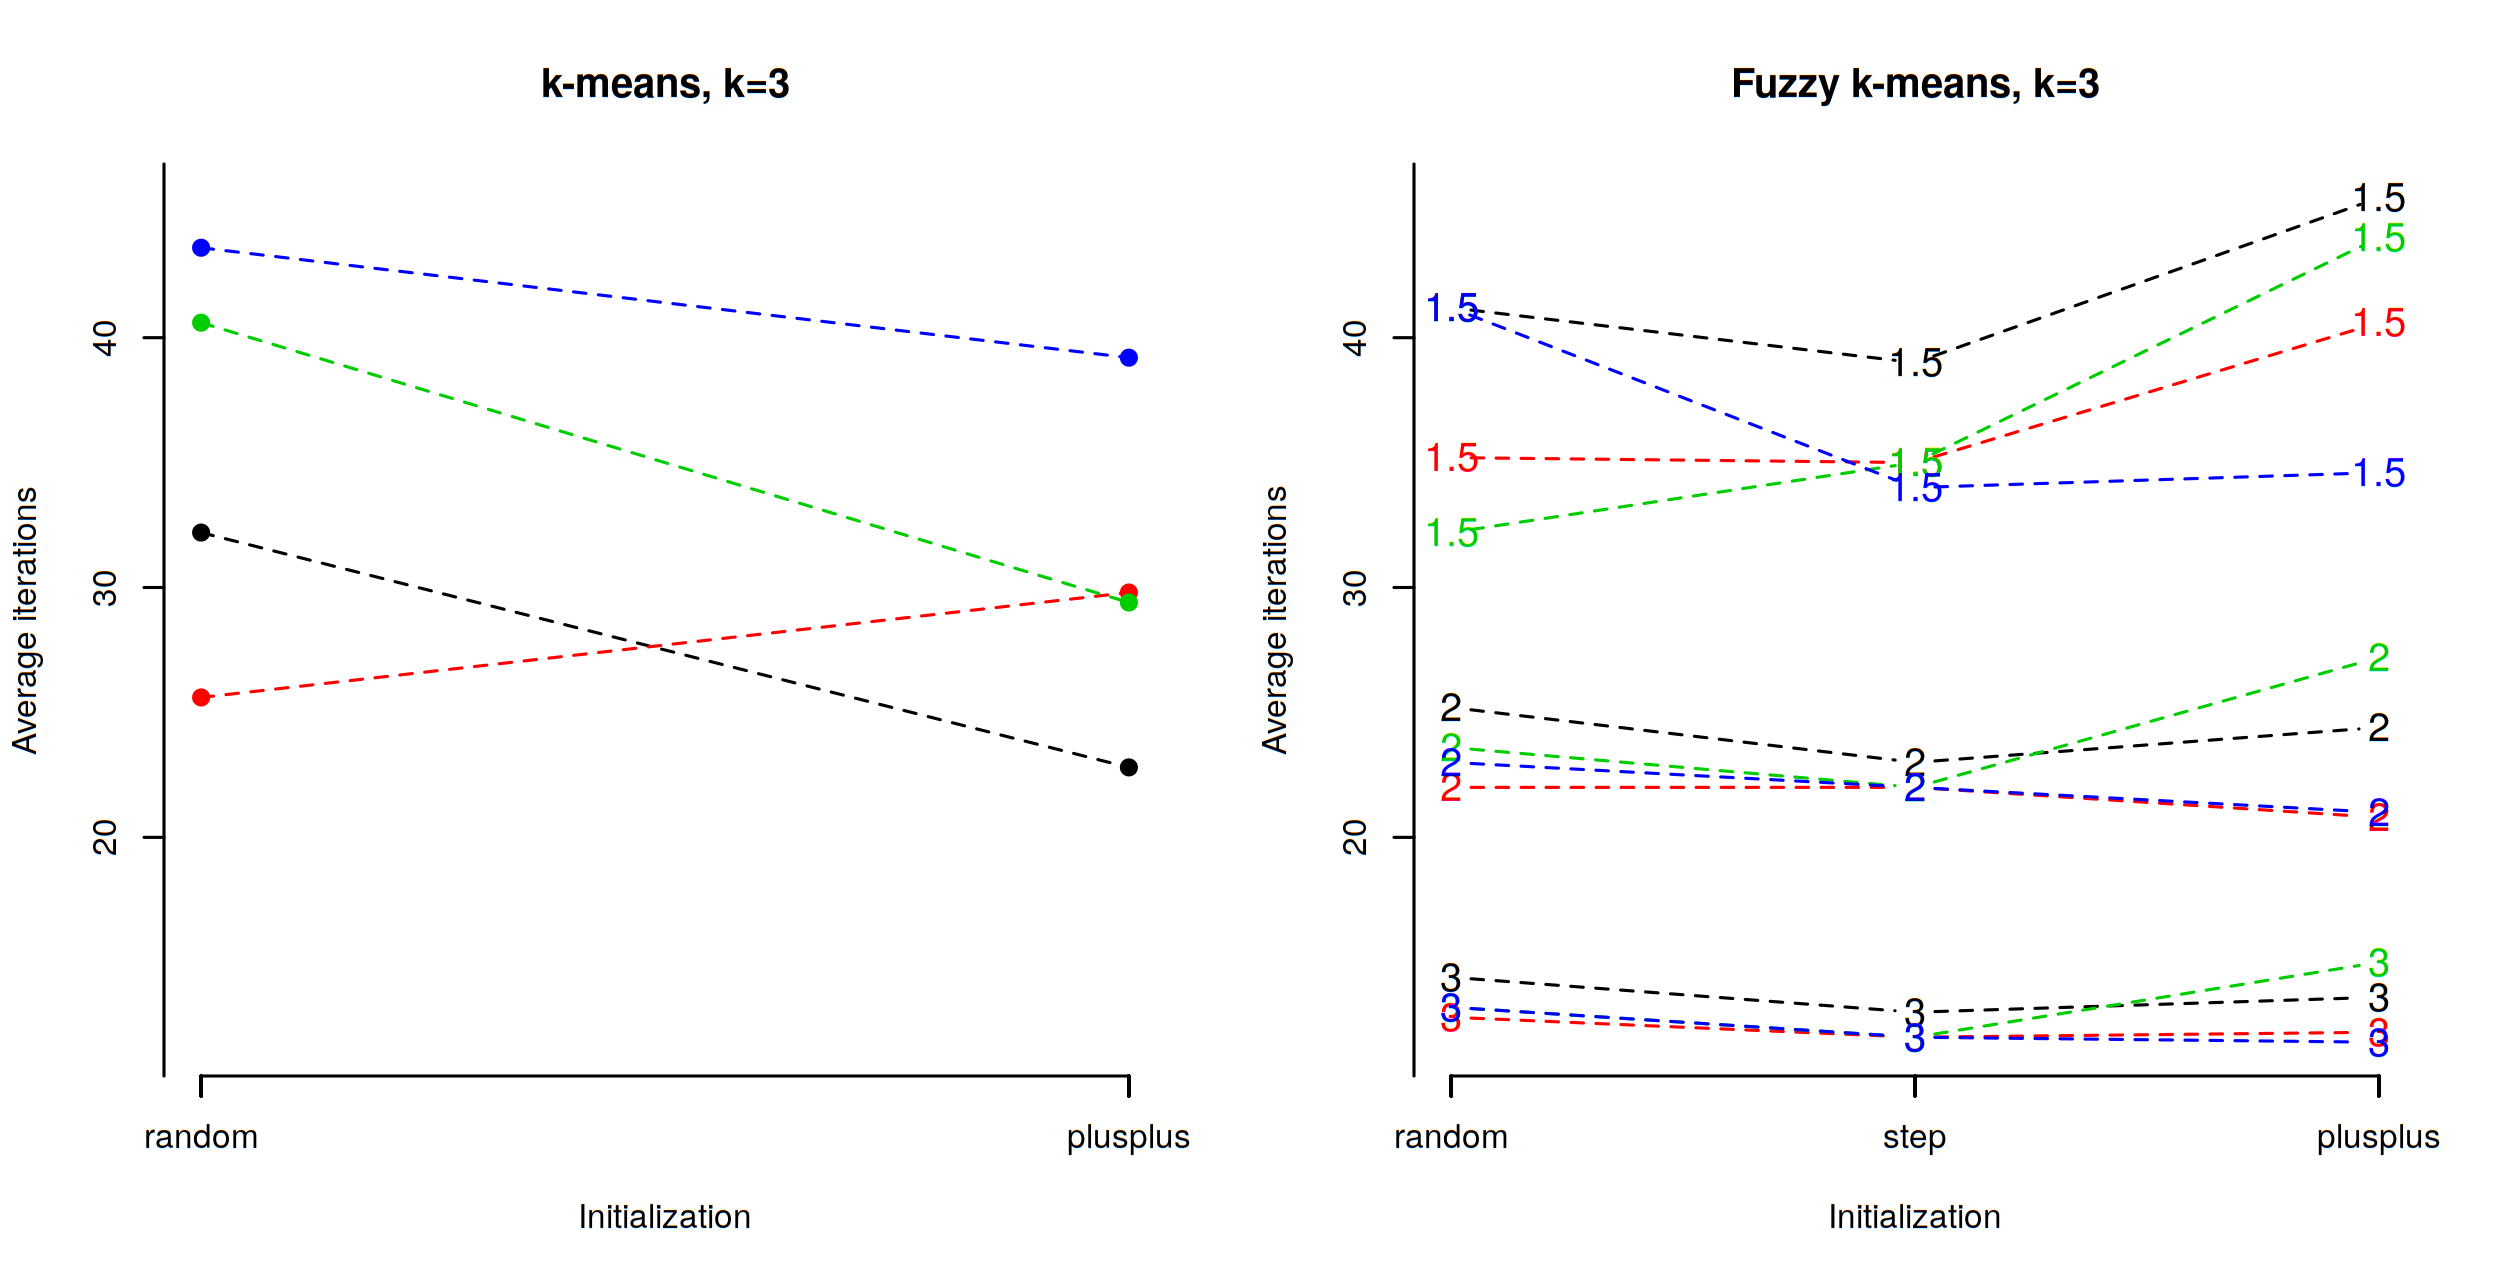
\includegraphics[width=0.99\textwidth]{figures/clust-3.png}
        \caption{Prove empiriche sui dataset di dimensione 15000 (\textit{nero}), 30000 (\textit{rosso}), 70000 (\textit{verde}), 115000 (\textit{blu}). Per il \fcm\ è indicato nel grafico il valore di $m$.}
        \label{fig:k3}
    \end{figure}
\end{frame}

\begin{frame}{Prove empiriche}
    \begin{figure}[H]
        \centering
        % trim l b r u
        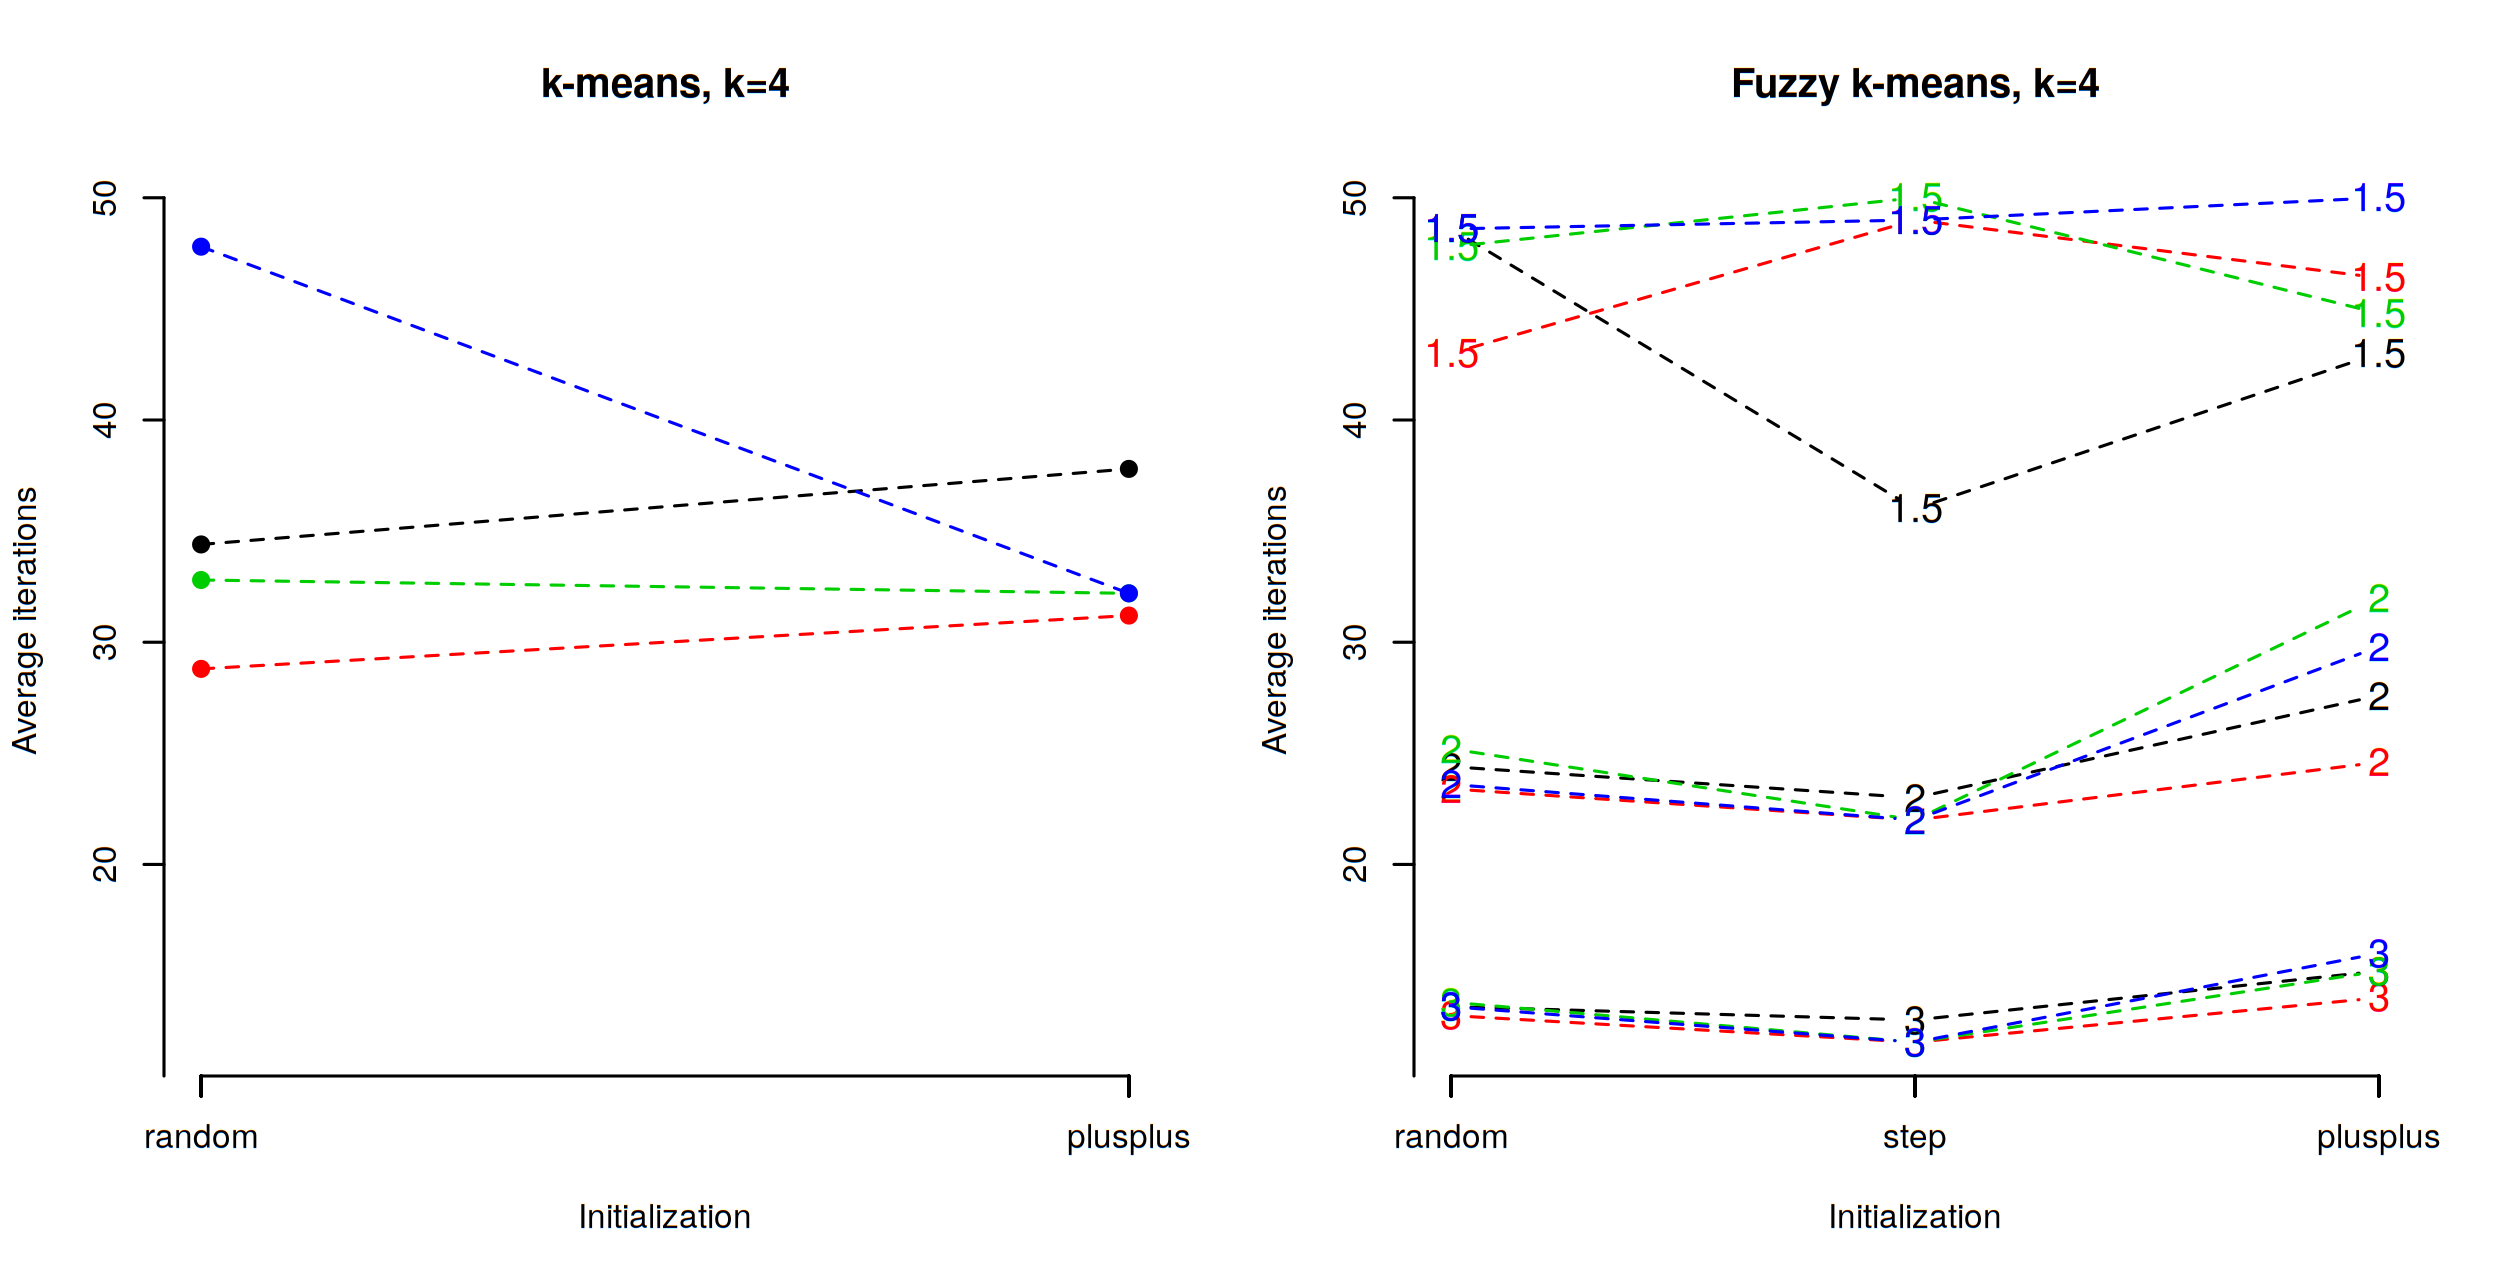
\includegraphics[width=0.99\textwidth]{figures/clust-4.png}
        \caption{Prove empiriche sui dataset di dimensione 15000 (\textit{nero}), 30000 (\textit{rosso}), 70000 (\textit{verde}), 115000 (\textit{blu}). Per il \fcm\ è indicato nel grafico il valore di $m$.}
        \label{fig:k4}
    \end{figure}
\end{frame}

\begin{frame}{Prove empiriche}
    \begin{figure}[H]
        \centering
        % trim l b r u
        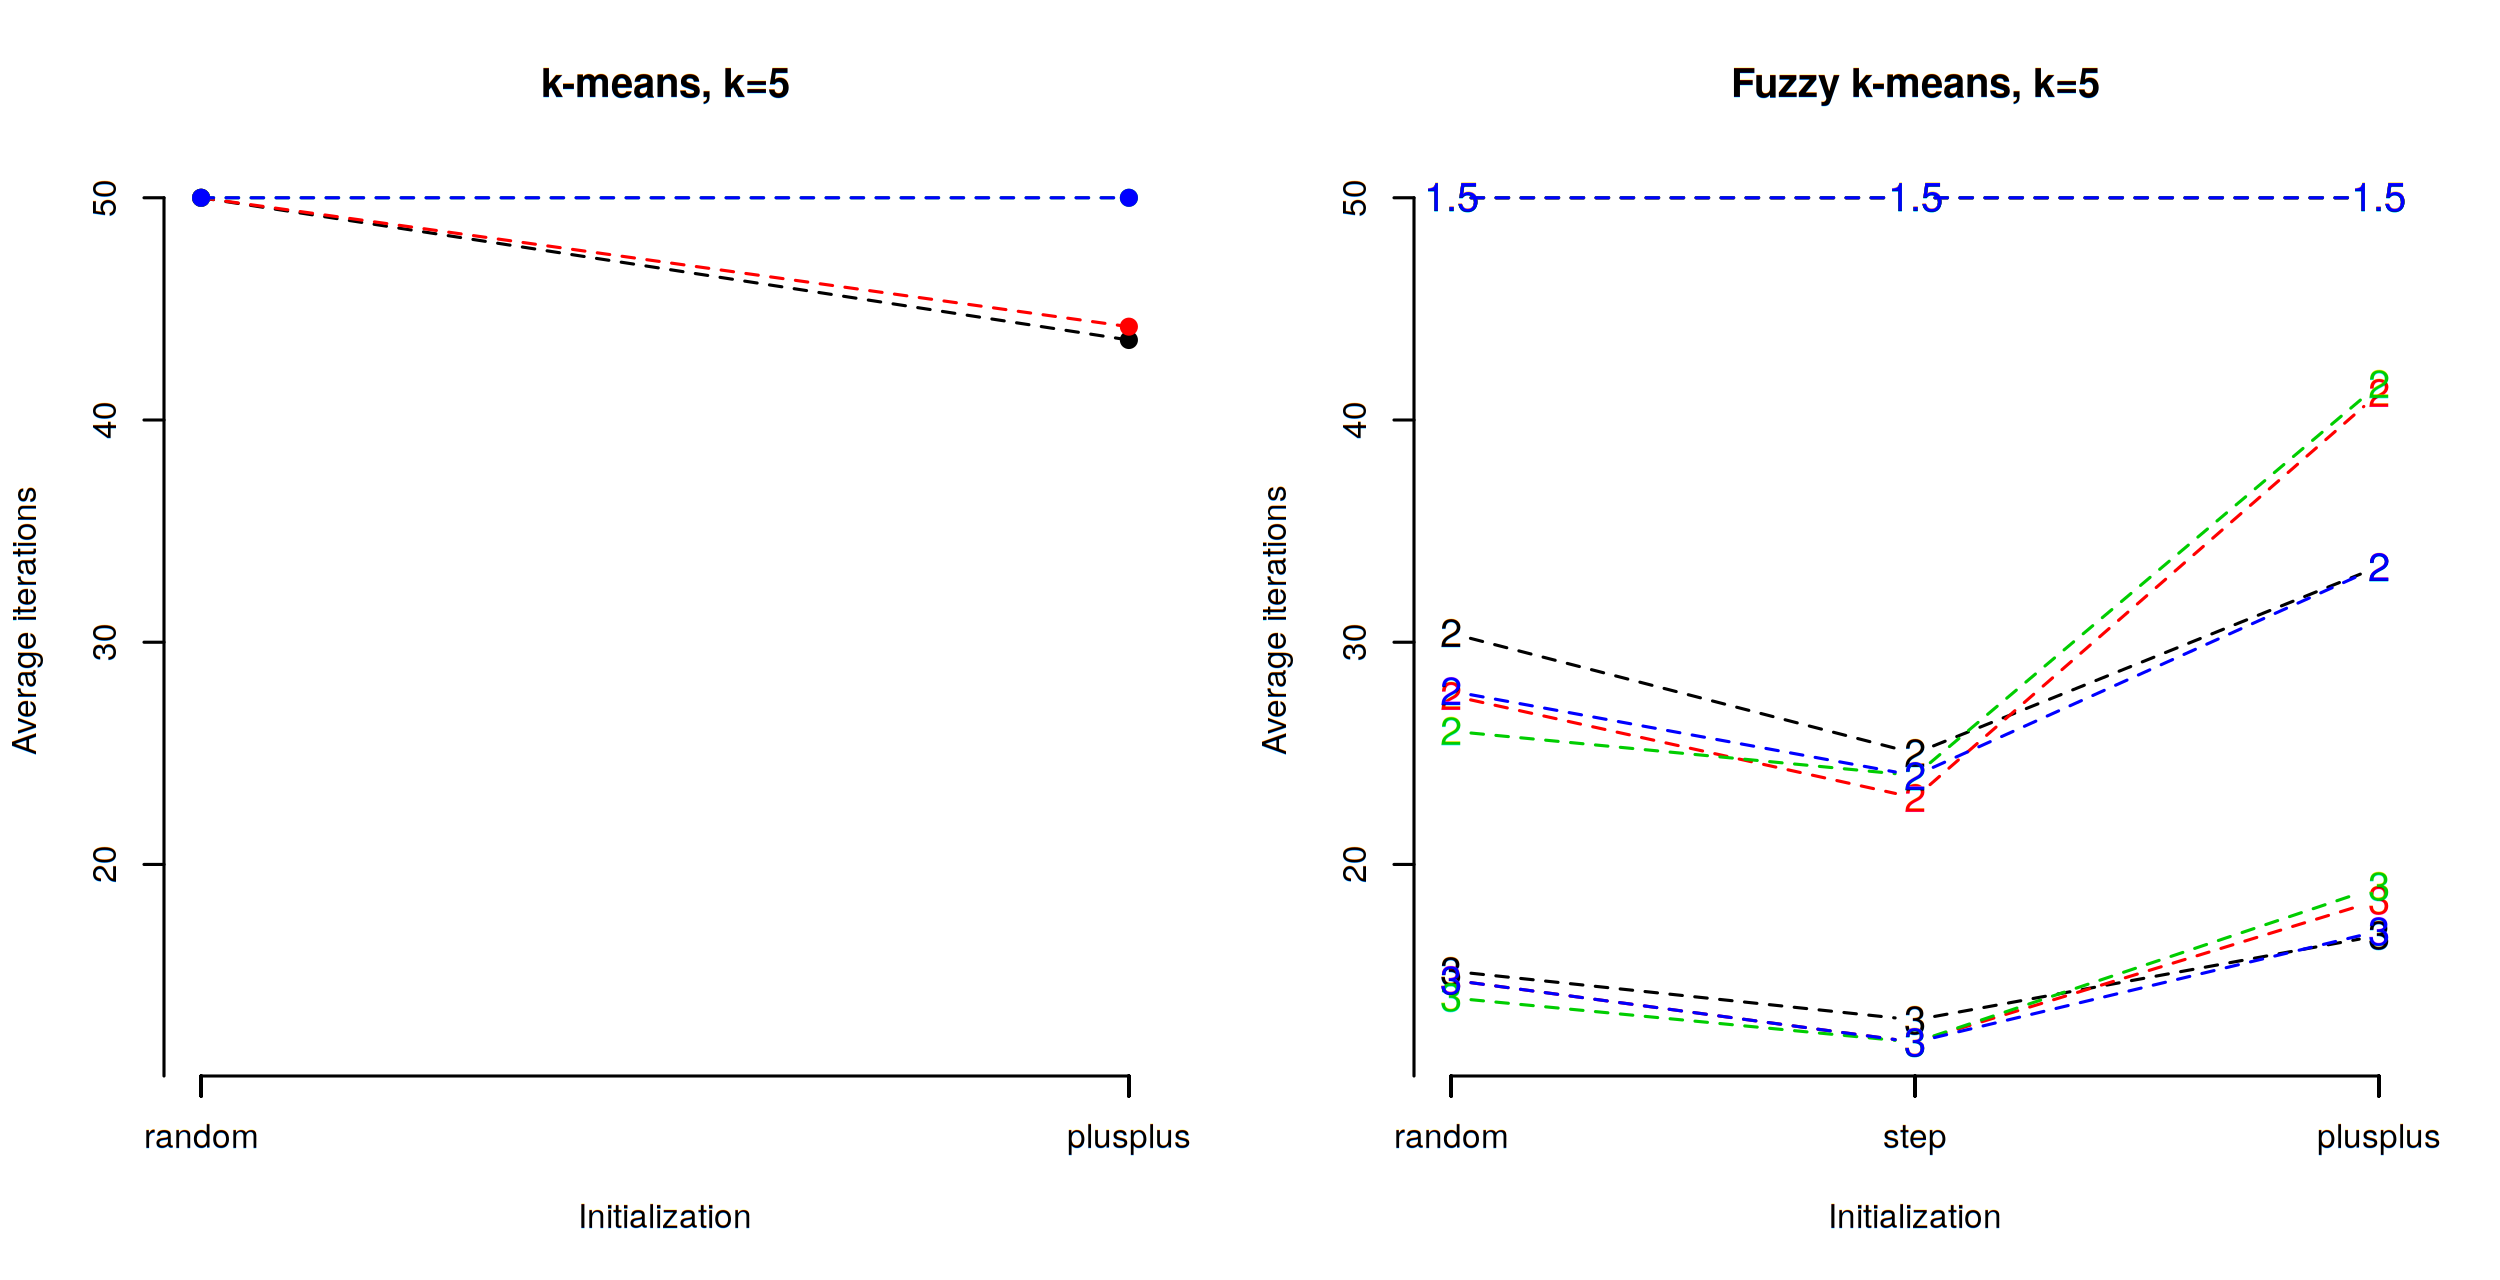
\includegraphics[width=0.99\textwidth]{figures/clust-5.png}
        \caption{Prove empiriche sui dataset di dimensione 15000 (\textit{nero}), 30000 (\textit{rosso}), 70000 (\textit{verde}), 115000 (\textit{blu}). Per il \fcm\ è indicato nel grafico il valore di $m$.}
        \label{fig:k5}
    \end{figure}
\end{frame}
% \bibliographystyle{splncs04}
% \bibliography{progetto}
\end{document}
